% 2021年北京高考数学第15题解析图1：y=|lg x|与直线
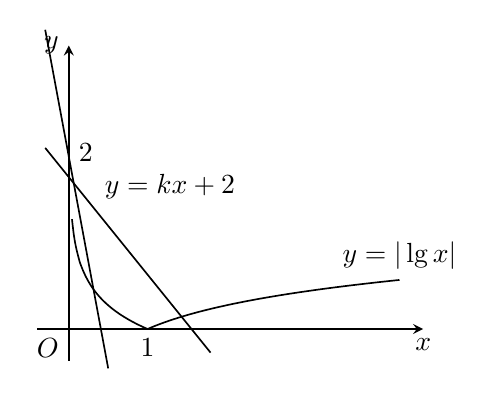
\begin{tikzpicture}[>=stealth,line width=0.6pt,font=\normalsize]
  \draw[->] (-0.4,0) -- (4.5,0) node[below] {$x$};
  \draw[->] (0,-0.4) -- (0,3.6) node[left] {$y$};
  \node[below left] at (0,0) {$O$};
  \node[below] at (1,0) {$1$};
  \node[above right] at (0,2) {$2$};

  % y = |lg x| 曲线
  \draw[domain=0.04:1,smooth,samples=50] plot (\x, {-ln(\x)/ln(10)});
  \draw[domain=1:4.2,smooth,samples=50] plot (\x, {ln(\x)/ln(10)}) node[above] {$y=|\lg x|$};

  % 两条过 (0,2) 的割线
  \draw (-0.3, 2.3) -- (1.8, -0.3) node[above right,pos=0.3] {$y=kx+2$};
  \draw (-0.3, 3.8) -- (0.5, -0.5);
\end{tikzpicture}
